\section{Planning Approach Methods}
The trip avoidance control we propose involves (1) estimating the position and
orientation of the leg (\cref{sec:hip_kalman}), (2) predicting the future hip
angles and heights (\cref{sec:predict_gp}), and (3) planning corresponding knee
and ankle trajectories such that the heel and toe will not contact the ground
prematurely (\cref{sec:traj_plan}).

\subsection{Extended Kalman Filter for estimating Leg Position/Orientation}
\label{sec:hip_kalman}

To estimate the position and orientation of the leg, we employ an EKF that fuses
information from a LIDAR distance sensor (SICK OD1000), an IMU (YEI Technologies
3-Space sensor), and encoders on the prosthesis (Renishaw Resolute, Netzer
DS-25). The EKF filters the nonlinear, discrete-time dynamics given by
\begin{align}
    x_{t} = \begin{bmatrix} q_t \\ p_t \\ \dot{p}_t \end{bmatrix}
        &= \begin{bmatrix} f_\tn{gyro}(\omega_t) & 0 & 0 \\
            0 & I_{3\times3} & \Delta t  I_{3\times3}\\
            0 & 0 & I_{3\times3} \end{bmatrix} x_{t-1} \notag \\
        &\quad+ \begin{bmatrix} 0 \\ \frac{1}{2} \Delta t^2 I_{3\times3} \\ 
            \Delta t I_{3\times3} \end{bmatrix} 
        \begin{bmatrix} R_\tn{OI}(q_{t-1}) a_t - \begin{bmatrix} 0 \\ 0 \\ g 
            \end{bmatrix} \end{bmatrix} + w_t \label{eq:dynamics}\\
            &= f(x_{t-1}, u_t) + w_t  \notag ,
\end{align}
where $q$ is the quaternion orientation, $R_\tn{OI}$ and $p$ are the rotation
matrix and position of the IMU in inertial coordinates, $\omega$ is the angular
rate measured by the gyroscope, $f_\tn{gyro}$ integrates the gyroscope rate to
update the orientation, $a$ is the accelerometer measurement, $u_t =
\left[\omega_t, a_t \right]^T$, and $\Delta t$ is the integration time step
(\unit[1]{ms}). 

The dynamics are corrupted by process noise $w_t \sim \mathcal{N}(0, Q_t)$ due
to the inaccuracy of the IMU's measurement of the true acceleration and angular
velocity. Consequently, $Q_t$ is given by
\begin{align}
    Q_t = \left. \frac{\partial f}{\partial u} \right|_{x_{t-1}, u_t}
        \begin{bmatrix} \sigma_\omega^2 I_{3\times3} & 0 \\ 
            0 & \sigma_a^2 I_{3\times3} \end{bmatrix}
        \left. \frac{\partial f}{\partial u} \right|_{x_{t-1}, u_t}^T,
\end{align}
where $\sigma_\omega^2$ and $\sigma_a^2$ are the gyroscope and accelerometer
measurement variances, respectively.

\begin{marginfigure}
    \centering
    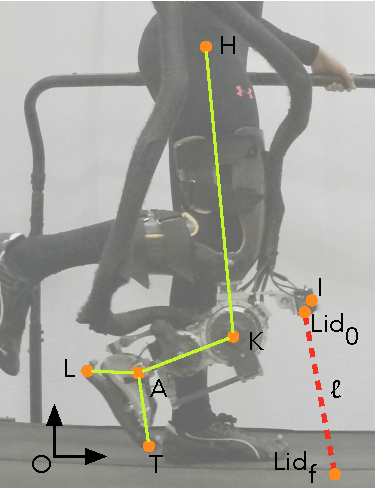
\includegraphics[width=\columnwidth]{kinematics}
    \caption[Kinematic model of the user and prosthesis used for state
    estimation and motion planning]{Kinematic model of the user and prosthesis
    used for state estimation and motion planning. The model includes the hip
    (H), knee (K), ankle (A), heel (L) and toe points (T). Additionally, the
    start ($Lid_0$) and end ($Lid_f$) points of the LIDAR beam (with length
    $\ell$) are indicated. The IMU is located at point $I$. Both the LIDAR and
    IMU are mounted to the thigh portion of the powered knee-and-ankle
    prosthesis.}\label{fig:kinematics}
\end{marginfigure}

To estimate the pose given our sensor measurements, we follow a standard EKF
procedure \citep{anderson1979optimal}, reviewed here for completeness. The EKF
state estimation process has two steps: First, we \emph{predict} the next state
distribution by forward-propagating the mean $\hat{x}_{t-1|t-1}$ and covariance
of the state estimate $\Sigma_{t-1|t-1}$ using the dynamics given by
\cref{eq:dynamics},
\begin{align}
    \hat{x}_{t|t-1} &= f(\hat{x}_{t-1|t-1}, u_t) \\
    \Sigma_{t|t-1} &= F_t \Sigma_{t-1|t-1} F_t^T + Q_t,
\end{align}
where $F_t = \left. \partial f / \partial x \right|_{\hat{x}_{t-1|t-1}}$.

Next, we incorporate information from noisy sensor observations to \emph{update}
the state estimate. To do this, we utilize a observation model given by $z_t =
h(x_t) + v_t$, where $v_t \sim \mathcal{N}\left(0, R \right)$, and the following
update equations:
\begin{align}
    K_t &= \Sigma_{t|t-1} H_t^T 
        {\left(H_t \Sigma_{t|t-1} H_t^T + R\right)}^{-1} \\
    \hat{x}_{t|t} &= \hat{x}_{t|t-1} + K_t \left(z_t - h(\hat{x}_{t|t-1}) \right) \\
    \Sigma_{t|t} &= \left(I - K_t H_t \right) \Sigma_{t|t-1}
\end{align}
where $z_t$ are the actual sensor measurements and $H_t = \left. \partial h /
\partial x \right|_{\hat{x}_{t-1|t}}$.

The observations in our EKF formulation use the kinematic model shown in
\cref{fig:kinematics}. We calibrate this model using ground truth data from a
VICON motion capture system. In our application we incorporate three
observations:
\begin{enumerate}
\item The expected acceleration vector points up in the global coordinate frame,
\begin{align} 
    h_1(x_t) &= {\left\{R_\tn{OI}(q) \right\}}_\textrm{row 3} \\
    z_1 &= a
\end{align}

\item The expected LIDAR measurement given the position of the IMU,
\begin{align}
    h_2(x_t) &= \left\{\ell : \left\{ p_\tn{OLID_f}\left(x_t, \ell \right)
        \right\}_\tn{row 3} = 0\right\} \\
    z_2 &= \ell_\tn{meas},
\end{align}
where $p_\tn{OLID_f}$, is the location of the laser beam endpoint represented in
the global coordinate system, $\ell = \lVert
\overrightarrow{\tn{LID_0}\tn{LID_f}} \rVert$ is the modeled laser beam length,
and $\ell_\tn{meas}$ is the actual measured LIDAR distance.

\item During stance, the toe point coincides with the origin (active
\unitfrac[200]{m}{s} after stance begins until toe-off)
\begin{align}
    h_3(x_t) &= p_\tn{OT}(x_t, \theta_\tn{k}, \theta_\tn{a}) \\
    z_3 &= {[0 \ 0 \ 0]}^T
\end{align}
where $p_\tn{OT}$ is the location of the toe in the inertial frame, and
$\theta_\tn{k}$ and $\theta_\tn{a}$ are the measured knee and ankle angles.
\end{enumerate}

The measurement noise for these observations is given by
\begin{align}
    R = \begin{bmatrix} \sigma_a^2 I_{3\times3} & 0 \\
        0 & \sigma_l^2 \end{bmatrix}
\end{align}
during swing and
\begin{align}
    R = \begin{bmatrix} \sigma_a^2 I_{3\times3} & 0 & 0 \\
        0 & \sigma_\ell^2 & 0 \\
        0 & 0 & \sigma_f^2 I_{3\times3} \end{bmatrix}
\end{align}
during stance. In these equations, $\sigma_a^2$ is the accelerometer variance,
$\sigma_\ell^2$ is the LIDAR measurement variance, and $\sigma_f^2$ is the foot
position variance.

To further improve the EKF's state estimate, we enforce a number of
constraints using the methods provided by \citet{gupta2007kalman}. Specifically,
we enforce three equality constraints:
\begin{enumerate}
\item First, we require that the quaternion has unit norm
\begin{align}
    1 = q_1^2 + q_2^2 + q_3^2 + q_4^2.
\end{align}

\item Second, we prevent the yaw component of the orientation $q$ from drifting.
To do this, we convert the $q$ to ZYX Euler angles and enforce $\phi_z = 0$, 
\begin{align}
    0 = \func{atan2}{2 (q_1 q_4 + q_2 q_3), 1 - 2 (q_3^2 + q_4^2)}.
\end{align}

\item Finally, during stance we further constrain the toe's $x$ and
$y$-coordinates to 0,
\begin{align}
    \begin{bmatrix} 0 \\ 0 \end{bmatrix} 
        &= {\left\{p_\tn{OT}(x_t, \theta_\tn{k}, \theta_\tn{a}) 
            \right\}}_\textrm{rows 1 and 2}.
\end{align}
\end{enumerate}

\noindent In addition, we use inequality constraints to ensure the toe and heel
do not penetrate the ground,
\begin{align}
    0 &\le {\left\{p_\tn{OT}(x_t, \theta_\tn{k}, \theta_\tn{a}) 
        \right\}}_\textrm{row 3} ,\\
    0 &\le {\left\{p_\tn{OL}(x_t, \theta_k, \theta_a) 
        \right\}}_\textrm{row 3}.
\end{align}

\noindent We enforce these constraints by solving the following quadratic
program after each update step,
\begin{align}
\hat{x}_{t|t}^\tn{proj} 
    &= {\argmin_x \left(x - \hat{x}_{t|t} \right)}^T \Sigma_{t|t}^{-1} 
        \left(x - \hat{x}_{t|t} \right),
\end{align}
such that
\begin{align}
    A_\tn{eq} x &= b_\tn{eq}, \\
    A_\tn{ineq} x &= b_\tn{ineq},
\end{align}
where $A_\tn{eq}$,  $b_\tn{eq}$, $A_\tn{ineq}$, and $b_\tn{ineq}$ are derived
from linearizing the equality and inequality constraints.

\begin{marginfigure}[-1in]
    \centering
    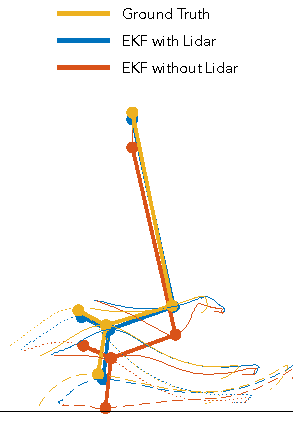
\includegraphics[width=\columnwidth]{ekf_fig}
    \caption[Trajectories of extended Kalman Filter (EKF) estimate of the
    position of the leg during swing compared to ground truth data from motion
    capture system]{Trajectories of extended Kalman Filter (EKF) estimate of the
    position of the leg during swing (blue). Ground truth positions given by
    motion capture (yellow). EKF estimate without LIDAR information shown in
    red. Thick lines show the leg configuration at peak toe height during swing.
    Dotted lines indicate heel trajectories while dashed lines show the toe
    trajectories. Knee and ankle trajectories given by solid
    lines.}\label{fig:ekf}
\end{marginfigure}

To identify the appropriate parameters of the Kalman filter, we collected ground
truth training and testing kinematic data using a Vicon motion capture system
and optimized the parameters of the EKF to minimize the error of the kinematic
estimate. The parameters we optimized were the rotation of the LIDAR with
respect to the hip, the translation between the LIDAR and the IMU, and
$\sigma_\omega$, $\sigma_a$, $\sigma_\ell$, and $\sigma_f$. 

\Cref{fig:ekf} shows an example of the resulting EKF estimates of the hip, knee,
ankle, heel, and toe positions during swing (blue stick figure and traces)
compared to the ground truth obtained from the motion capture system (yellow)
and an EKF estimate without the LIDAR sensor information integrated (red). Over
the entire test data set, the root mean squared error of the estimated heel and
toe positions during swing is \unit[18.6]{mm} for the EKF with LIDAR
information. In contrast, the EKF without LIDAR information has an error of
\unit[46.7]{mm}. Thus, including the LIDAR sensor data reduces the error by
60\%.

\begin{figure}[t]
    \centering
    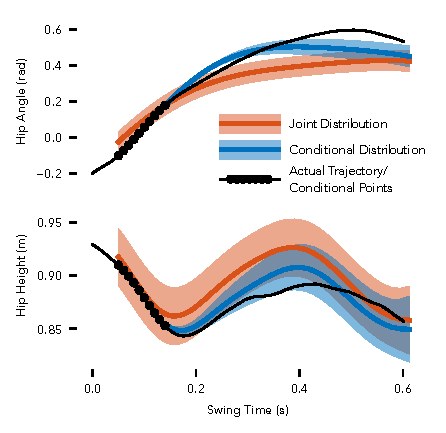
\includegraphics[width=\columnwidth]{gp_plots_w_legend}
    \caption[Example of hip angle and height trajectory predictions]{Example of
    hip angle and height trajectory predictions \unit[0.15]{s} into swing. The
    prediction algorithm uses the previous 10 measured hip angles and heights
    (sampled at \unit[100]{Hz}, black dots) along with the learned joint
    distributions of hip angles/heights versus time (red) to obtain the
    conditional distributions of future hip angles/heights (blue). The planning
    algorithm uses the means of the conditional distributions to generate knee
    and ankle trajectories. The actual hip height and angle trajectories are
    shown in black.}\label{fig:gp_plots}
\end{figure}
\subsection{Gaussian Process Hip Trajectory Prediction}

\label{sec:predict_gp}
To predict the future hip angle and height trajectories, we train sparse
Gaussian process models using the FITC approximation \citep{snelson2007local}.
The sparse approximation ensures the computational complexity at test time is
independent of the training data set size, providing consistent real time
performance. Throughout the swing phase, the learned hip angle and height
distributions are conditioned on the swing trajectories completed so far to
predict the distribution of the future trajectories for the rest of the swing
(example shown in \cref{fig:gp_plots}). Our algorithm then uses the means of
these conditional distributions in the motion planning phase
(compare \cref{sec:traj_plan}). 

For example, to calculate the conditional mean of future hip angles, we first
compute the joint distribution of completed $(\theta_h^\tn{c})$ and future
$(\theta_h^\tn{f})$ hip angles,
\begin{align}
    \func{P}{\theta_h^\tn{c}, \theta_h^\tn{f}} &=
        \mathcal{N}\left(\mu_\tn{fitc}, \Sigma_\tn{fitc} 
            + K\left( t_\tn{joint}, t_\tn{joint} \right) \right) \\
    &= \mathcal{N}\left( 
        \begin{bmatrix} 
            \mu_\tn{c} \\ \mu_\tn{f} 
        \end{bmatrix},
        \begin{bmatrix} 
            \Sigma_{\tn{c},\tn{c}} & \Sigma_{\tn{c},\tn{f}} \\ 
            \Sigma_{\tn{f},\tn{c}} & \Sigma_{\tn{f},\tn{f}} 
        \end{bmatrix}
        \right),
\end{align}
where $\mu_\tn{fitc}$ and $\Sigma_\tn{fitc}$ are obtained from equation 11 in
\citep{snelson2007local} and $K\left( t_\tn{joint}, t_\tn{joint}\right)$ is an
additional noise term given by a rational quadratic kernel
\citep{rasmussen2004gaussian} that correlates the predicted angles across time,
which results in smooth predicted trajectories. The mean of the conditional
distribution $\func{P}{\theta_h^\tn{f}|\theta_h^\tn{c}}$ is then given by
\begin{align}
    \mu_\tn{f}^\tn{cond} = \mu_\tn{f} + \Sigma_{\tn{f},\tn{c}}
        \Sigma_{\tn{c},\tn{c}}^{-1}\left(\mu_\tn{c} - \theta_h^\tn{c} \right).
    \label{eq:gp_cond_mean}
\end{align}
As the inversion of $\Sigma_{\tn{c},\tn{c}}$ is the most computationally
expensive component of \cref{eq:gp_cond_mean}, we use at most the last 10 hip
angles and heights (sampled at \unit[100]{Hz}) when calculating the conditional
mean (compare \cref{fig:gp_plots}).

\subsection{Trajectory Planning Quadratic Program Formulation}
\label{sec:traj_plan}

\begin{pagefigure}
    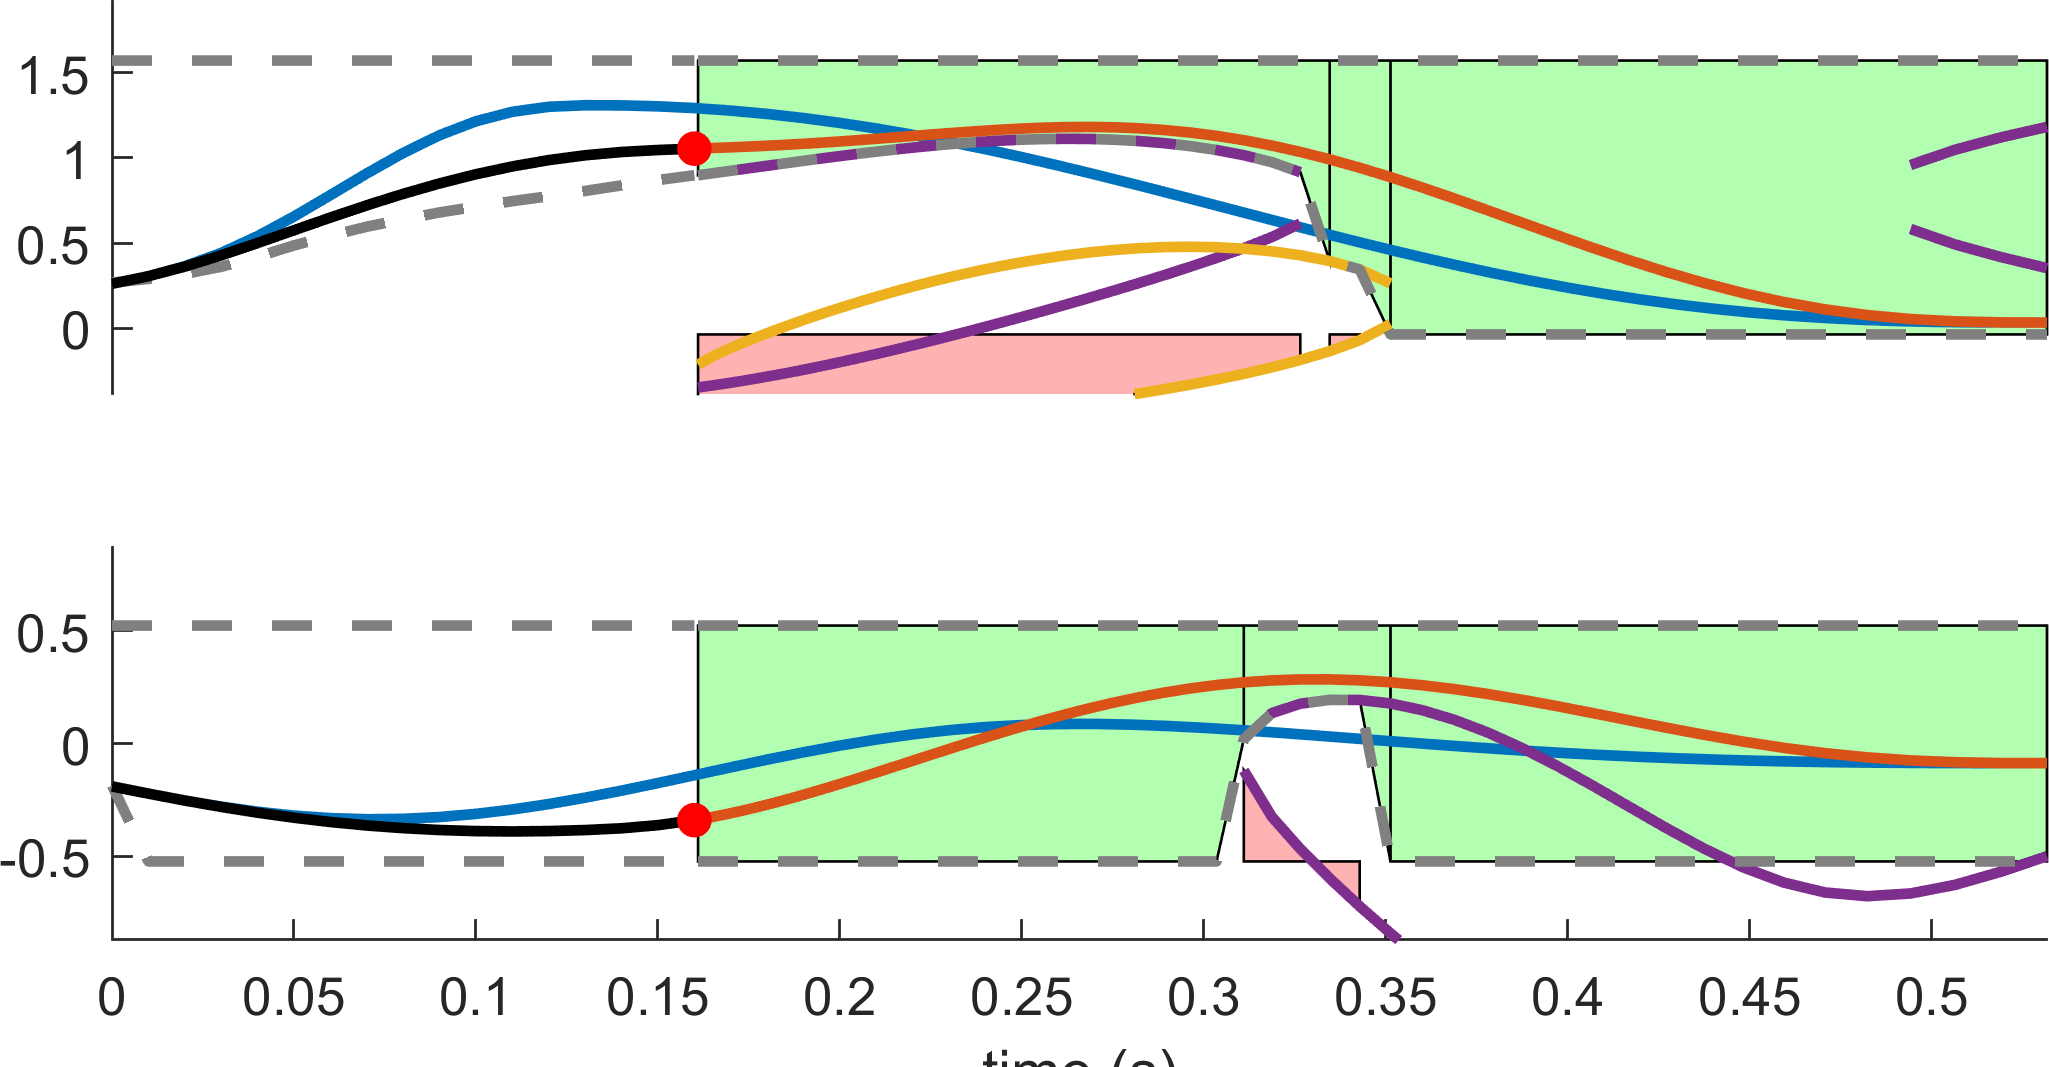
\includegraphics[width=\textwidth]{planning}
    \caption[Planning Algorithm Steps]{Planning Algorithm Steps: Panels B and D
    show the generated knee and ankle trajectories respectively.  The planned
    trajectory (red) lies within the computed bounds (dashed gray).  In
    contrast, standard minimum jerk trajectories (blue) do not respect the
    bounds, thereby increasing the tripping hazard. Panels C and E show examples
    of inverse kinematics (IK) solutions for toe (purple) and heel (yellow)
    contact for the knee and ankle joints respectively. We use the IK solutions
    to generate bounded regions that the planned trajectory can safely traverse.
    We consider ground contact constraints for only the first half of the
    remaining swing duration after which we only consider joint angle
    constraints. We use Dijkstra's algorithm to select regions (green) that
    allow a path from the start point to the desired final point. Bounded
    regions that do not lie on the path are shown in red. Panel A shows the
    corresponding prosthesis motion.}\label{fig:planning}
\end{pagefigure}

To obtain reactive control of the prosthesis swing leg motion, we plan future
swing trajectories with a fast quadratic program (QP) operating at
\unit[100]{Hz}. The QP includes equality constraints, which ensure the
trajectories progress smoothly from the current position to the desired end
position, and inequality constraints, which avoid premature ground contact of
toe and heel of the prosthesis. Because in our formulation the QP can only solve
for one joint at a time, we first solve for the ankle trajectory assuming the
knee trajectory found in the previous time step, and then use this updated ankle
trajectory to solve for the new knee trajectory.

\Cref{fig:planning} provides more details of the actions of the trajectory
planner algorithm. For example, at a time of about \unit[150]{ms} into the swing
phase, the algorithm solves
\begin{align}
    \theta_\tn{k}^\textrm{toe bnd} 
        &= \left\{\theta_\tn{k} : \left\{p_\tn{OT}
            (\theta_\tn{h}, z_\tn{h}, \theta_\tn{k}, \theta_\tn{a})
            \right\}_\textrm{row 3} = 0 \right\} \\
    \theta_k^\textrm{heel bnd} 
        &= \left\{\theta_\tn{k} : \left\{p_\tn{OL}
            (\theta_\tn{h}, z_\tn{h}, \theta_\tn{k}, \theta_\tn{a})
            \right\}_\textrm{row 3} = 0 \right\}
\end{align}
at a set of sample times spanning the remaining swing trajectory to obtain a
planned knee trajectory (red trace in \cref{fig:planning}B).
Figures~\cref{fig:planning}C and E show the predicted inverse kinematics (IK)
solutions at characteristic points into the swing for the knee and ankle
respectively, with solutions leading to toe contact shown in purple and
solutions leading to heel contact shown in yellow. For each contact point, there
are typically two solutions, one lower bound, for which the joint angle cannot
cross from above, and one upper bound, for which the joint angle cannot cross
from below. 

Often, the valid leg configurations span disjointed regions in the configuration
space (green and red regions in \cref{fig:planning}B and D). Therefore, the
planner next identifies a valid sequence of regions for the trajectory to
traverse in a four step procedure.  First, the planner identifies critical
points along the predicted trajectory at which any bound activates or
deactivates. Second, at each critical point, the planner sorts the bound angles
from largest to smallest and iterates through them to define regions between
successive upper and lower bounds. Third, the planner defines a graph over the
regions with edge weights equal to the average squared angle minus the volume of
the child region. This cost favors a sequence of regions that are large and thus
safe to travel trough and avoids regions that require excessive joint flexion or
extension. Dijkstra's algorithm is then used to find a valid sequence of regions
that minimizes this cost~\citep{dijkstra1959note}. Finally, so that the
generated trajectories do not get too close to the identified bounds, a buffer
is added to the bounds. This buffer takes the form
\begin{align}
    \theta_\tn{buf} = \theta_\tn{buf}^0 \sin 
        \left(\pi \frac{t - t_0}{t_f - t_0} \right),
\end{align}
where $\theta_\tn{buf}^0$ is either \unit[5]{$^\circ$} or \unit[-5]{$^\circ$}
for lower and upper bounds respectively, $t$ is the future swing time, and $t_0$
and $t_f$ are the current and final swing times.

After identifying the bounded regions, the planner generates the trajectory for
a specific joint by solving a quadratic program. The trajectory of each joint is
represented by three, fifth-order polynomial splines,
\begin{align}
    \theta_1(t) &= a_{01} + a_{11} t + \cdots + a_{51} t^5 
        = [1 \ t \cdots t^5] a_1 \\ 
        T_0 &\le t < T_1 \\
    &\vdots \notag \\
    \theta_3(t) &= a_{03} + a_{13} t + \cdots + a_{53} t^5 
        = [1 \ t \cdots t^5] a_3 \\ 
     T_2 &\le t < T_F,
\end{align}
and solved for by the following QP,
\begin{align}
    a^* = \argmin_a \ \frac{1}{2} a^T (H_\theta + w H_{\dddot{\theta}}) a
    \label{eq:quadprog},
\end{align}
where $a = [a_1^T \ a_2^T \ a_3^T]^T$, $H_\theta$ and $H_{\dddot{\theta}}$
encode quadratic costs on angle and jerk respectively, and $w$ is a weight
parameter. The solution is subject to the inequality constraints
\begin{align}
    \theta(t) &\le \theta_\tn{max}(t), \ \forall t\\
    \theta(t) &\ge \theta_\tn{min}(t), \ \forall t\\
    \dot{\theta}(t) &\le \dot{\theta}_\tn{max}, \ \forall t\\
    \dot{\theta}(t) &\ge \dot{\theta}_\tn{min}, \ \forall t,
\end{align}
which ensure the trajectory lies within the identified bounds and respects
velocity limits, and to the equality constraints
\begin{align}
\theta(T_0) &= \theta_0 \\
\dot{\theta}(T_0) &= \dot{\theta}_0 \\
\ddot{\theta}(T_0) &= \ddot{\theta}_0 \\
\theta(T_F) &= \theta_F \\
\dot{\theta}(T_F) &= 0 \\
\ddot{\theta}(T_F) &= 0 \\
\theta_1(T_1) &= \theta_2(T_1) \\
\dot{\theta}_1(T_1) &= \dot{\theta}_2(T_1) \\
\ddot{\theta}_1(T_1) &= \ddot{\theta}_2(T_1) 
\label{eq:quadprog_last_constraint} \\
&\vdots \notag
\end{align}
which ensure the trajectory starts at the current and terminates at the desired
positions, velocities, and accelerations and that the splines join together
smoothly.  If the QP fails to find a trajectory that can satisfy the
constraints, the last found valid trajectory is reused for the next time step.
In addition, at the first iteration, the ankle trajectory planner uses the
output of the minimum jerk trajectory planner to solve the inverse kinematics
for the bounds. 

\subsection{Experimental Procedure}
We tested the ability of the proposed trip avoidance control to reduce the
incidence and severity of trips while walking with the powered transfemoral
prosthesis shown in \cref{fig:kinematics} To evaluate the performance of the
system, an able-bodied user walked with the prosthesis while attempting to
elicit trips by lowering the hip in swing. During the stance phase, the
prosthesis randomly decided to either use the proposed swing control or to use
standard minimum jerk trajectories that do not consider the tripping hazard. The
user was not aware of which controller would be used in the upcoming swing.  The
user completed a total of ten one minute walking trials.

We examined several outcomes for evaluating the control performance. First, we
examined the distribution of knee angles at the beginning of stance. Large knee
angles at the beginning of stance indicate premature landing due to toe-strike
instead of heel strike. Ideally, the landing angle is close to the desired final
angle of \unit[2]{degrees}. Second, we checked the integral of the ground
reaction force during swing. If this quantity is large, it indicates scuffing of
the toe on the ground. Finally, we examined the relationship between the hip and
toe heights during swing. If our controller is working as intended, the toe
height during swing should have a decreased sensitivity to the hip height.
